\section{Results}
After running our hybrid decision tree algorithm over the various settings of training, tuning, and testing sets, we generate learning curves to compare the performance of standard decision trees (in which a leaf's associated prediction is based on a plurality of the subset of training data at that leaf) and our hybrid trees.  In Figure \ref{fig:learn_curve}, we can see that the performance of standard trees actually fell off with increased training set size, which provides evidence of overfitting. The hybrid trees, in contrast, showed great improvements in accuracy relative to the standard trees, with the margin increasing for larger training and tuning sets.

\begin{figure}
	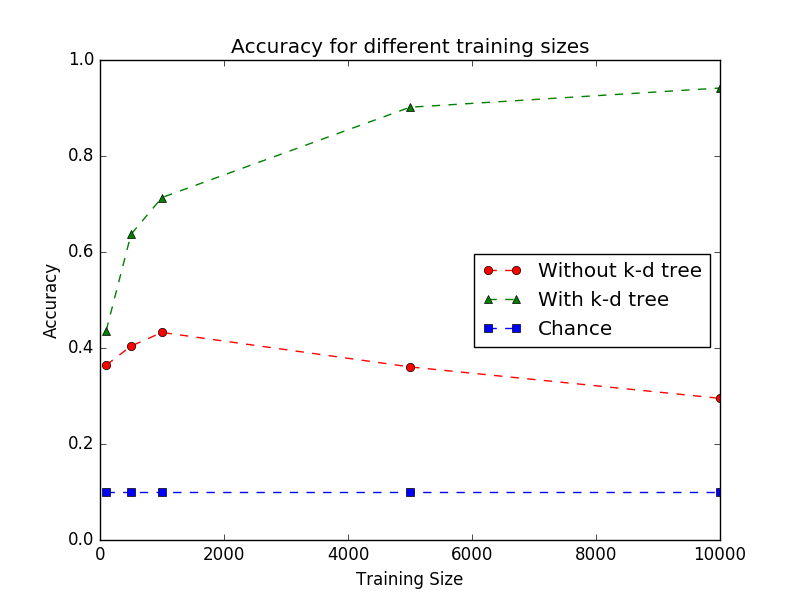
\includegraphics[width=\linewidth]{Figures/learning_curve.png}
	\caption{Learning curve for standard decision trees and hybrid trees with k-d trees.  Note that the chance line assumes a uniform distribution of the 10 handwritten digits.}
	\label{fig:learn_curve}
\end{figure}

To assess the classifier's performance for each handwritten digit, we used the predictions from the setting with 10000 training examples (1000 tuning examples and 10000 testing) to generate a confusion matrix and calculate the values of precision and recall for each digit.  Again, we repeated this for both standard and hybrid decision trees.  Looking at Table \ref{table:no_kd_precision_recall} we can see the digit 2 was never predicted by the standard decision tree.  Other digits, such as 9, exhibit extremely low values of recall. Looking at the confusion matrix in Table \ref{table:no_kd_confusion} we see that the standard decision tree classifier most often predicted the digit 7 for a handwritten 9.  We also have some digits the exhibit unusually low precision coupled with good recall.  For example, the standard decision tree classifier often predicted 1 when presented with examples of other handwritten digits.

Looking at Table \ref{table:with_kd_confusion} and Table \ref{table:with_kd_precision_recall} we can see that the handwritten 2 is actually classifiable (has non-zero precision and recall) by the hybrid classifier.  Additionally, Table \ref{table:with_kd_precision_recall} does not exhibit those unusually low values of precision and recall

\begin{table}
	\begin{tabular}{l|llllllllll}
		&   '0' &   '1' &   '2' &   '3' &   '4' &   '5' &   '6' &   '7' &   '8' &   '9' \\
		\hline
		'0' &   368 &     3 &     2 &     0 &     1 &     4 &     3 &     2 &     0 &     2 \\
		'1' &   517 &  1128 &   444 &   968 &    87 &   742 &   146 &   133 &   866 &    87 \\
		'2' &     8 &     0 &     0 &     0 &     0 &     0 &     0 &     0 &     0 &     0 \\
		'3' &     0 &     0 &     0 &     1 &     0 &     0 &     0 &     0 &     0 &     0 \\
		'4' &     4 &     0 &     1 &     0 &     1 &     0 &     0 &     0 &     3 &     0 \\
		'5' &     8 &     0 &     0 &     2 &     0 &     1 &     0 &     0 &     0 &     0 \\
		'6' &    42 &     4 &   536 &    21 &    18 &    45 &   561 &     5 &    17 &     3 \\
		'7' &    33 &     0 &    49 &    18 &   874 &   100 &   248 &   888 &    86 &   916 \\
		'8' &     0 &     0 &     0 &     0 &     1 &     0 &     0 &     0 &     2 &     0 \\
		'9' &     0 &     0 &     0 &     0 &     0 &     0 &     0 &     0 &     0 &     1 \\
	\end{tabular}
	\caption{Confusion matrix for standard decision trees.  Note that horizontal indices correspond to the actual labels of the handwritten digits while vertical indices correspond to the labels predicted by the tree.}
	\label{table:no_kd_confusion}
\end{table}

\begin{table}
	\centering
	\begin{tabular}{rrr}
		Digit &   Precision &      Recall \\
		\hline
		0 &   0.955844  & 0.37551     \\
		1 &   0.220399  & 0.993833    \\
		2 &   0         & 0           \\
		3 &   1         & 0.000990099 \\
		4 &   0.111111  & 0.00101833  \\
		5 &   0.0909091 & 0.00112108  \\
		6 &   0.448083  & 0.585595    \\
		7 &   0.276463  & 0.863813    \\
		8 &   0.666667  & 0.00205339  \\
		9 &   1         & 0.00099108  \\
	\end{tabular}
	\caption{Precision and recall for standard decision trees, for each handwritten digit.}
	\label{table:no_kd_precision_recall}
\end{table}

\begin{table}
	\begin{tabular}{l|llllllllll}
		&   '0' &   '1' &   '2' &   '3' &   '4' &   '5' &   '6' &   '7' &   '8' &   '9' \\
		\hline
		'0' &   940 &     3 &    12 &     0 &     1 &    11 &     8 &     2 &     8 &     7 \\
		'1' &     3 &  1125 &     7 &     1 &     9 &     4 &     3 &    22 &     2 &     7 \\
		'2' &    10 &     2 &   965 &     9 &     1 &     0 &     0 &     7 &     7 &     2 \\
		'3' &     0 &     2 &    12 &   944 &     0 &    25 &     1 &     1 &    33 &     7 \\
		'4' &     4 &     0 &     5 &     1 &   909 &     1 &     4 &     4 &     9 &    16 \\
		'5' &    12 &     0 &     1 &    22 &     0 &   813 &     2 &     1 &    16 &     3 \\
		'6' &     8 &     3 &     3 &     3 &     9 &    19 &   938 &     0 &     7 &     0 \\
		'7' &     3 &     0 &    20 &     7 &     7 &     8 &     0 &   975 &     6 &    19 \\
		'8' &     0 &     0 &     6 &    12 &     2 &     7 &     2 &     0 &   864 &     5 \\
		'9' &     0 &     0 &     1 &    11 &    44 &     4 &     0 &    16 &    22 &   943 \\
	\end{tabular}
	\caption{Confusion matrix for new hybrid decision trees.  Note that horizontal indices correspond to the actual labels of the handwritten digits while vertical indices correspond to the labels predicted by the tree.}
	\label{table:with_kd_confusion}
\end{table}

\begin{table}
	\centering
	\begin{tabular}{rrr}
		\hline
		Digit &   Precision &   Recall \\
		0 &    0.947581 & 0.959184 \\
		1 &    0.950972 & 0.991189 \\
		2 &    0.962114 & 0.935078 \\
		3 &    0.920976 & 0.934653 \\
		4 &    0.95383  & 0.925662 \\
		5 &    0.934483 & 0.911435 \\
		6 &    0.947475 & 0.979123 \\
		7 &    0.933014 & 0.948444 \\
		8 &    0.962138 & 0.887064 \\
		9 &    0.90586  & 0.934589 \\
	\end{tabular}
	\caption{Precision and recall for hybrid decision trees, for each handwritten digit.}
	\label{table:with_kd_precision_recall}
\end{table}